\chapter{\textit{Frameworks} MVC e de Persistência}\label{cap:frameworksPersistencia}
\epigraph{``\textit{A persistência é o caminho do êxito}''.}{Charles Chaplin}
\epigraph{``\textit{Não extingua sua inspiração e sua imaginação; não se torne o escravo do seu modelo}''.}{Vincent van Gogh}

\lettrine[lines=4, lhang=0.1, lraise=0, loversize=0.2, findent=0.1em]{\textcolor{corTema}{N}}{ESTE} Capítulo reconstruiremos o ``Sistema de Venda de Produtos'' do Capítulo~\ref{cap:terceiroProjeto} utilizando diversos \textit{frameworks} que tornarão nosso trabalho menos tedioso e mais direto ao ponto!

\vfill

\section{Introdução}

Antes de começarmos a trabalhar, precisamos configurar nosso ambiente de desenvolvimento. Como lidaremos com toda a \textit{stack} de \textit{frameworks} e bibliotecas do Spring, poderíamos utilizar a ferramenta oficial deles para nos auxiliar, a Spring Tool Suite 4. Eu particularmente não sou muito fã, pois ela é baseada na IDE Eclipse que, na minha opinião, é extremamente burocrática e instável, mas como ela é adotada como o padrão da indústria, uma hora ou outra acabamos ter que a adotar. Continuaremos a utilizar o NetBeans como nossa ferramenta padrão, mas você pode testar a Spring Tool Suite caso deseje. No momento em que este texto está sendo escrito existem também versões para o Visual Studio Code (\url{https://code.visualstudio.com/}) a para a IDE Theia (\url{https://theia-ide.org/}). O download de qualquer uma das versões pode ser feito em \url{https://spring.io/tools}.

A primeira coisa que vamos fazer é acessar o site Spring Initializr (\url{https://start.spring.io/}). Nesse site podermos configurar a infraestrutura básica do nosso projeto, que utilizará o Maven (\url{https://maven.apache.org/}) como ferrameta de gerenciamento do projeto. O Maven é suportado atualmente pelas principais IDEs disponíveis. Sendo um projeto Maven, espera-se que todas as IDEs trabalhem de forma semelhante, então teoriacemente podemos trabalhar com mais de uma ferramenta no mesmo projeto. Note que iremos reconstruir o ``Sistema de Venda de Produtos'' do Capítulo\ref{cap:terceiroProjeto}. Vamos começar?

A versão atual da página principal do site do Spring Initializr pode ser vista na Figura~\ref{fig:cap10SpringInitializr}.

\FloatBarrier
\begin{figure}[!htbp]
    \centering
    \caption{Tela principal do site do Spring Initializr}
    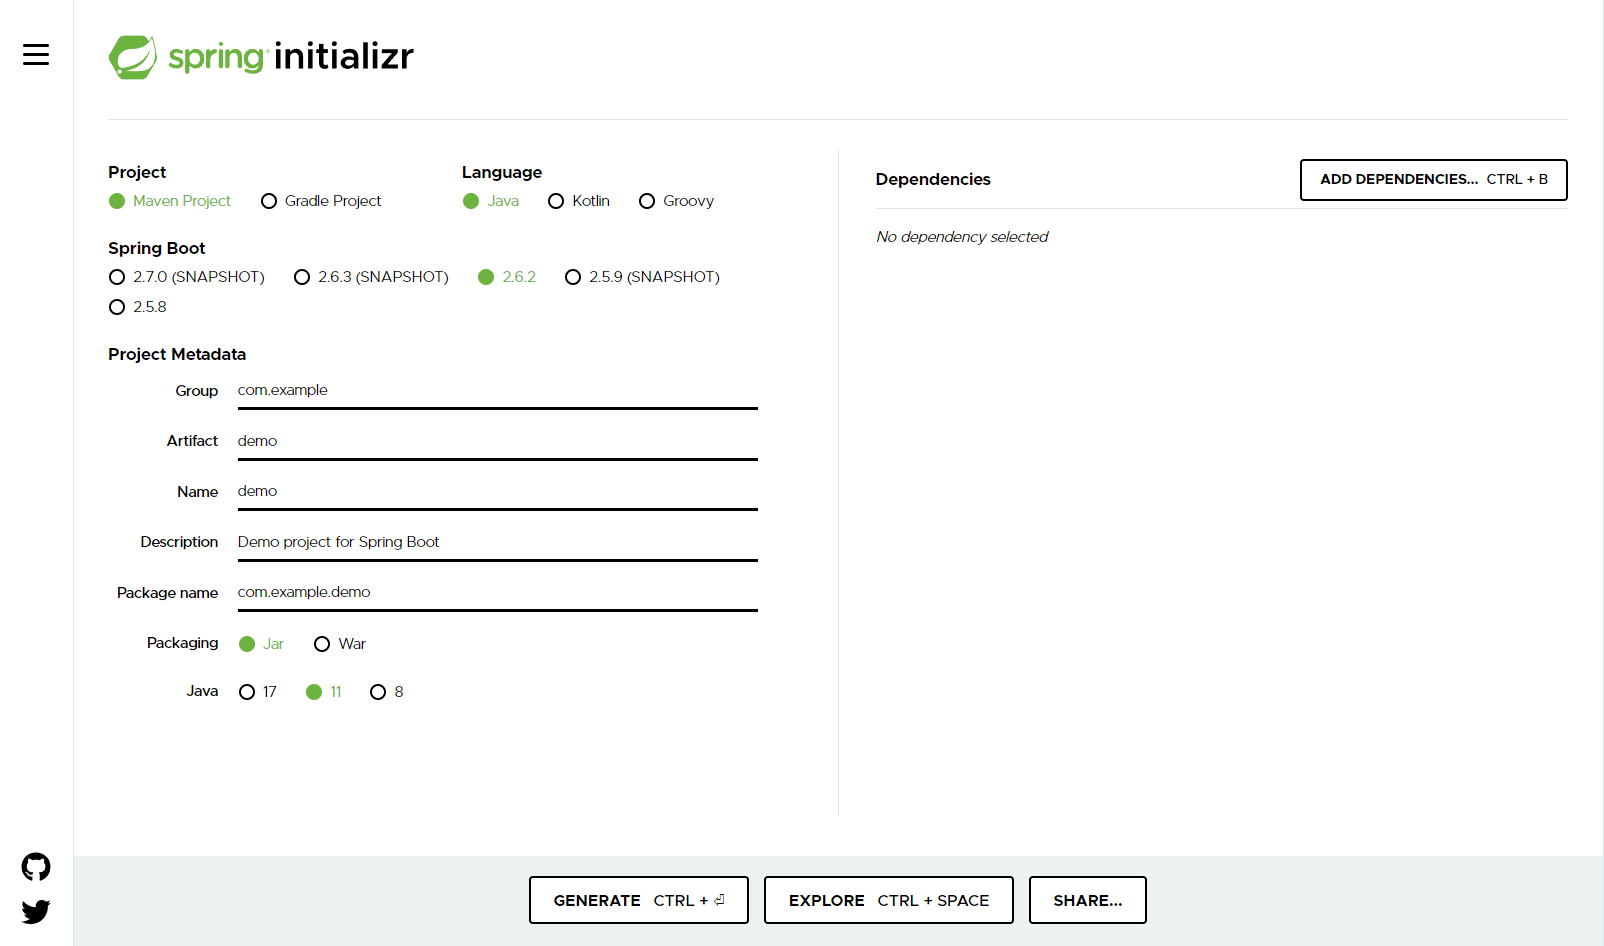
\includegraphics[scale=0.4]{imagens/cap10SpringInitializr}
    \\\textbf{Fonte:} \url{https://start.spring.io/}
    \label{fig:cap10SpringInitializr}
\end{figure}
\FloatBarrier

Basicamente do lado esquerdo temos as opções de configuração do projeto:

\begin{itemize}
    \item \textbf{\textit{Project}:} qual ferramenta de gerencimanto de projetos que será usada (usaremos o Maven);
    \item \textbf{\textit{Language}:} a linguagem de programação utilizada no projeto;
    \item \textbf{\textit{Spring Boot}:} qual a versão do Spring Boot que usaremos;
    \item \textbf{\textit{Project Metadata}:} os metadados do projeto, que envolvem:
    \begin{itemize}
        \item \textbf{\textit{Group}:} nome do identificador do grupo do projeto, normalmente igual ao pacote da organização/empresa do desenvolvedor do projeto, seguindo as regras para noemação de pacotes da linguagem Java (\url{https://docs.oracle.com/javase/specs/jls/se6/html/packages.html#7.7});
        \item \textbf{\textit{Artifact}:} nome do arquivo que será gerado (sem a extensão \texttt{.jar} ou \texttt{.war}) após a construção do projeto e também o identificador que será usado pelo Maven para encontrar a versão compilada e instalada do projeto dentro do repositório local do Maven. Normalmente identificador do artefato tiver mais de uma palavra, separamos as mesmas por hífens;
        \item \textbf{\textit{Name}:} nome do projeto, o que aparecerá na raiz do projeto aberto nas IDEs para identificá-los;
        \item \textbf{\textit{Description}:} breve descrição do objetivo do projeto;
        \item \textbf{\textit{Project name}:} pacote raiz do projeto, usando como prefixo o identificador do grupo. Caso sejam usados hífens~\footnote{O Spring Initializr usará automaticamente o valor do identificador artefato aqui, trazendo hífens, que serão descartados no pacote final}, eles serão suprimidos no projeto gerado;
        \item \textbf{\textit{Packaging}:} tipo de empacotamento que será feito. Arquivos \texttt{.jar} podem ser executados localmente e arquivos \texttt{.war} são destinados à implantação em servidores de aplicações e/ou containeres de Servetls;
        \item \textbf{\textit{Java}:} a versão do Java que se quer usar. Note que apenas as versões \textit{Long-Term Support} (LTS) aparecem e, além disso, você precisa ficar atento para ter um JDK de versão igual ou superior instalado na máquina de desenvolvimento.
    \end{itemize}
\end{itemize}

Sabendo disso, vamos agora preparar o nosso projeto de acordo com o apresentado na Figura~\ref{fig:cap10SpringInitializrConfProjeto01}:

\FloatBarrier
\begin{figure}[!htbp]
    \centering
    \caption{Definição das propriedades do projeto}
    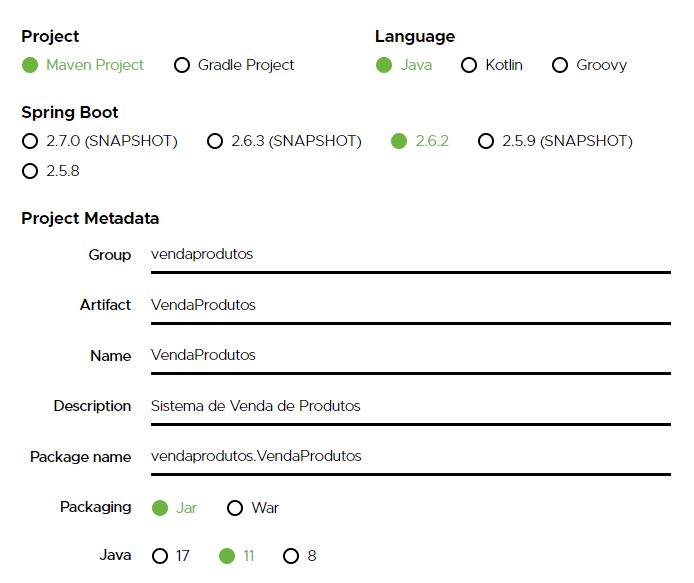
\includegraphics[scale=0.7]{imagens/cap10SpringInitializrConfProjeto01}
    \\\textbf{Fonte:} \url{https://start.spring.io/}
    \label{fig:cap10SpringInitializrConfProjeto01}
\end{figure}
\FloatBarrier

Ou seja:

\begin{itemize}
    \item \textbf{\textit{Project}:} usaremos o Maven;
    \item \textbf{\textit{Language}:} programaremos em Java;
    \item \textbf{\textit{Spring Boot}:} a última versão estável do Spring Boot, nesse caso, a 2.6.2. Note que isso pode variar de acordo com a época que você estiver lendo esse texto;
    \item \textbf{\textit{Project Metadata}:} os metadados do projeto, que envolvem:
    \begin{itemize}
        \item \textbf{\textit{Group}:} usaremos \texttt{dsoc7}, que é a sigla da disciplina para a qual esse livro foi desenvolvido incialmente, mas em um caso real, você deve preencher com a notação de domínio inverso da empresa ou instituição para a qual estiver desenvolvendo o projeto. Por exemplo, se a instuição tem o domínio \texttt{ifsp.edu.br}, você deverá preencher o identificador do grupo com \texttt{br.edu.ifsp}. Caso seja um projeto pessoal e você possuir um domínio, a regra é a mesma. Eu por exemplo tenho o domínio \texttt{davidbuzatto.com.br}, então meu identificador de grupo, para um projeto pessoal, deve ser \texttt{br.com.davidbuzatto};
        \item \textbf{\textit{Artifact}:} usaremos \texttt{venda-produtos-spring};
        \item \textbf{\textit{Name}:} o nome preencheremos com \texttt{VendaProdutosSpring}, que é o que aparecerá no NetBeans na raiz do projeto. Aqui em um caso real você poderia usar espaços para nomear o projeto. Eu prefiro sem espaços. Note que para diferenciar do primeiro projeto de venda de produtos, adicionaremos o sufixo Spring;
        \item \textbf{\textit{Description}:} preencher com Sistema de Venda de Produtos Usando Spring Boot;
        \item \textbf{\textit{Project name}:} aqui o Spring Initializr já deve ter preenchido com a concatenção do identificador do grupo e do identificador do artefato, ficando \texttt{dsoc7.venda-produtos-spring}. Na criação do projeto esses hífens serão retirados, pois nomes de pacotes em Java não podem ter hífem;
        \item \textbf{\textit{Packaging}:} usaremos empacotamento em \texttt{.jar};
        \item \textbf{\textit{Java}:} usaremos o Java 11.
    \end{itemize}
\end{itemize}

Com isso feito temos a configuração básica do projeto pronta, mas ainda precisamos adicionar as primeiras dependências que utilizaremos. As dependências são basicamente as biblitecas que usaremos no projeto. A vantagem de usar um sistema de gerenciamento de projetos como o Maven é que, ao adicionarmos dependências no projeto, ele se encarregará de carregar todas as dependências que uma dependência depende, inclusive com as versões apropriadas! Nossa vida fica muito mais fácil sem precisar ficar lidando com definição de bibliotecas e isso é um super avanço na produtividade!

Para adicionar uma dependência, clique no botão \destaque{\textit{ADD DEPENDENCIES...}}. Ao fazer isso, um diálogo aparecerá, onde você poderá escolher as dependências do projeto. Ao encontrar a dependência desejada, basta clicar nela que ela será inserida na lista de dependências do projeto. Você pode procurar pelas dependências rolando a lista ou então pesquisando na caixa de texto acima. No nosso projeto utilizaremos sete dependências, apresentadas na Figura~\ref{fig:cap10SpringInitializrConfProjeto02} e descritas a seguir.

\FloatBarrier
\begin{figure}[!htbp]
    \centering
    \caption{Definição das dependências do projeto}
    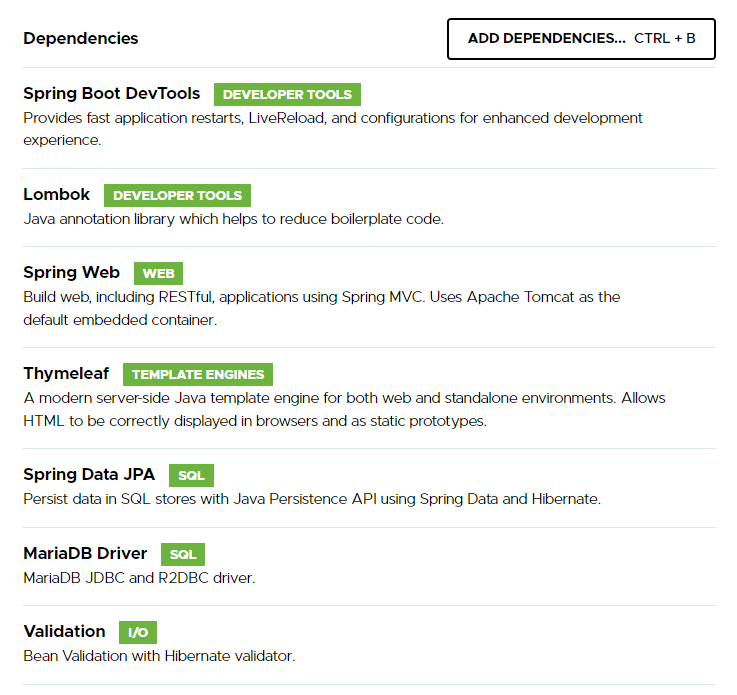
\includegraphics[scale=0.7]{imagens/cap10SpringInitializrConfProjeto02}
    \\\textbf{Fonte:} \url{https://start.spring.io/}
    \label{fig:cap10SpringInitializrConfProjeto02}
\end{figure}
\FloatBarrier

\begin{itemize}
    \item \textbf{Spring Boot DevTools:} auxília no desenvolvimento de aplicações usando Spring Boot, permitindo reinicialização rápida, integração com LiveReload etc;
    \item \textbf{Lombok:} é uma biblioteca de anotações que nos ajuda na criação automática de código padronizado como getters, setters, construtores etc;
    \item \textbf{Spring Web:} construção de aplicações Web usando o padrão de projeto MVC através do \textit{framework} Spring MVC, além da criação de Web Services RESTful;
    \item \textbf{Thymeleaf:} é uma \textit{template engine} que permite a definição de modelos para a criação de interfaces gráficas usando HTML, diminuindo a duplicidade de código e facilitando a manutenção.
    \item \textbf{Spring Data JPA:} \textit{framework} para persistência de dados usando Hibernate e a Java Persistence API (JPA);
    \item \textbf{MariaDB Driver:} driver de conexão com MariaDB, o SGBD que estamos utilizando neste livro;
    \item \textbf{Validation:} permite a validação de objetos de dados que serão gerenciados pela aplicação (já fizemos algo parecido, você se lembram?);
\end{itemize}

Agora com o inicializador do projeto configurado, clique no botão \destaque{\textit{GENERATE}}. Ao fazer isso, um arquivo \texttt{.zip} será baixado, com o nome de \texttt{venda-produtos-spring.zip}. No local onde foi salvo, descompacte-o. Abra o NetBeanse realize o procedimento de abrir projetos. Vá à pasta onde o arquivo foi descompactado. Você notará que o NetBeans reconhecerá um projeto Maven ali. Selecione-o e abra-o.

As configurações iniciais do projeto gerado no Spring Initilizr podem ser compartilhadas. Sendo assim, se você quiser, pode usar o \textit{link} abaixo para fazer o \textit{download} do projeto com as mesmas configurações apresentadas.

\url{https://start.spring.io/#!type=maven-project&language=java&platformVersion=2.6.2&packaging=jar&jvmVersion=11&groupId=dsoc7&artifactId=venda-produtos-spring&name=VendaProdutosSpring&description=Sistema%20de%20Venda%20de%20Produtos%20Usando%20Spring%20Boot&packageName=dsoc7.venda-produtos-spring&dependencies=devtools,lombok,web,thymeleaf,data-jpa,mariadb,validation}

Provavelmente, após abrir o projeto, seu NetBeans vai demorar alguns minutos --pode demorar bastante na verdade-- para baixar o índice central do Maven e prepará-lo no seu computador. Após esse processo, seu NetBeans vai ``reclamar'', informando que o repositório do Maven local não tem uma cópia das dependências do projeto. Veja na Figura~\ref{fig:cap10ConfProjeto03} o que provavelmente aparecerá, ou seja, um sinal de aviso (\textit{warning}) no ícone do projeto.

\FloatBarrier
\begin{figure}[!htbp]
    \centering
    \caption{Resolução de problema do projeto criado}
    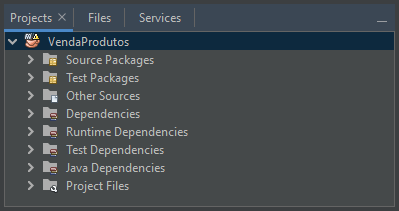
\includegraphics[scale=1]{imagens/cap10ConfProjeto03}
    \\\textbf{Fonte:} Elaborada pelo autor
    \label{fig:cap10ConfProjeto03}
\end{figure}
\FloatBarrier

Para resolvermos isso, faremos algo que talvez você já tenha feito para outras situações. Clique com o botão direito no projeto e escolha a opção \destaque{\textit{Resolve Project Problems...}} do menu de contexto. Fazendo isso, um diálogo aparecerá com um ou mais itens com o texto ``\textit{Some dependency artifacts are not in the local repository}'', indicando o problema encontrado. Clique no botão \destaque{\textit{``Resolve''}}. O Maven vai começar a realizar o processo de ``Priming'' (preparação) do projeto, prepararando e baixando todas as dependências. Essa preparação pode demorar um pouco também. Você saberá que o processo terminou quando aparecer ``BUILD SUCESS'' na saída do NetBeans e quando o diálogo da solução dos problemas do projeto apresentar o problema apontado anteriormente com um ``check'' ou ``tick'' verde. Clique em \destaque{\textit{Close}}.

Agora que criamos o projeto no Spring Initializr e o abrimos no NetBeans, vamos entender sua estrutura que é mostrada com seus principais nós expandidos na Figura~\ref{fig:cap10EstruturaProjeto}

\FloatBarrier
\begin{figure}[!htbp]
    \centering
    \caption{Estrutura do projeto}
    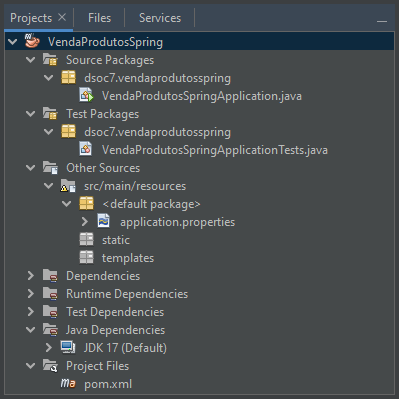
\includegraphics[scale=1]{imagens/cap10EstruturaProjeto}
    \\\textbf{Fonte:} Elaborada pelo autor
    \label{fig:cap10EstruturaProjeto}
\end{figure}
\FloatBarrier

As pastas \destaque{\textit{Source Packages}} e \destaque{\textit{Test Packages}} servirão para armazenar, respectivamente, arquivos de código e arquivos de teste do projeto. A pasta \destaque{\textit{Other Sources}} será usada para armazenar quaisquer outros tipos de arquivos do nosso projeto. Note que por padrão o NetBeans a mostrará como as outras duas pastas, ou seja, subentendendo que é uma pasta que conterá código em Java, mas isso não é verdade. Vamos mudar a aparência de como essa pasta é exibida para ficar parecido com o que estávamos acostumados na pasta Web dos nossos projetos anteriores, ou seja, uma exibição como uma árvore de diretórios, não de pacotes. Para isso, clique com o botão direito do mouse em \destaque{\textit{Other Sources}} e escolha a opção \destaque{\textit{Show Resources as Packages}} (Figura~\ref{fig:cap10ShowResourcesAsPackages}), desmarcando-a. 

\FloatBarrier
\begin{figure}[!htbp]
    \centering
    \caption{Estrutura do projeto}
    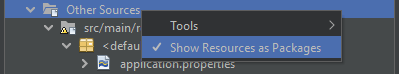
\includegraphics[scale=1]{imagens/cap10ShowResourcesAsPackages}
    \\\textbf{Fonte:} Elaborada pelo autor
    \label{fig:cap10ShowResourcesAsPackages}
\end{figure}
\FloatBarrier

Fazendo isso, a exibição dessa pasta se tornará a exibição padrão de árvore de diretórios, como mostrado na Figura\ref{fig:cap10EstruturaProjetoOK}. Dentro dela teremos inicialmente três itens: 1~) O diretório \destaque{\texttt{static}} que usaremos para armazenar todos os arquivos que conterão conteúdo estático; 2~) o diretório \destaque{\texttt{templates}} que conterá todos os \textit{templates} (modelos) que serão processados pelo \textit{framework} Thymeleaf e, 3~) o arquivo \destaque{\texttt{application.properties}} que armazenará todas as configurações que o Spring Boot usará para configurar todas as dependências do projeto. Eu sei que já começaram a aparecer algumas coisas que ainda não foram explicadas, mas não se preocupe que logo veremos a serventia de cada coisa.

\FloatBarrier
\begin{figure}[!htbp]
    \centering
    \caption{Estrutura do projeto}
    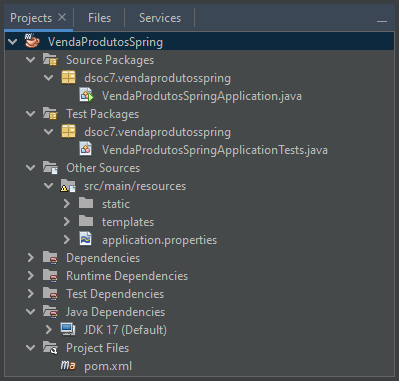
\includegraphics[scale=1]{imagens/cap10EstruturaProjetoOK}
    \\\textbf{Fonte:} Elaborada pelo autor
    \label{fig:cap10EstruturaProjetoOK}
\end{figure}
\FloatBarrier

Ainda sobre a estrutura do projeto, as pastas \destaque{\textit{Dependencies}}, \destaque{\textit{Runtime Dependencies}} e \destaque{\textit{Test Dependencies}} contém respectivamente as dependências de compilação, execução e teste. O conteúdo delas não serão exibidas, pois contém muitos itens e eles são gerenciados diretamente pelo Maven. Na pasta \destaque{\textit{Java Dependencies}} é mostrado qual o JDK está em uso, no meu caso o 17, sendo que pode ser qualquer um com versão maior ou igual à 11 e, em \destaque{\textit{Project Files}} há um arquivo denominado \destaque{\texttt{pom.xml}} que contém as configurações do Maven para o nosso projeto. Eu não mostrarei o conteúdo aqui, pois ele estará disponível para vocês. Abra-o para dar uma olhada no seu conteúdo e siga o texto para entender o que está acontecendo em algumas de suas partes.

Entre as linhas 5 e 10 é informado que este projeto é do tipo Spring Boot, versão 2.6.2, lembrando que a versão pode variar. Entre as linhas 11 e 18 são mostrados os valores correspondentes aos metadados que preenchemos no Spring Initializr, com uma única adição, a tag \inlineHTMLCode{<version>} usada para informar a versão do projeto. Por padrão, a versão inicial vem com o conteúdo \texttt{0.0.1-SNAPSHOT}. Se você quiser mudar esse valor, fique à vontade! Agora, entre as linhas 19 e 58 são definidas todas as dependências que escolhemos no Spring Initializr. Se quisermos adicionar mais dependências, podemos editar diretamente esse arquivo ou ir no Spring Initializr, escolher a dependência que queremos inserir como gerenciada pelo Spring Boot, clicar no botão \destaque{\textit{EXPLORE}}, copiar o trecho de código XML e colar no nosso arquivo \destaque{\texttt{pom.xml}}. Dependências que não são gerenciadas pelo Spring Boot também podem ser inseridas.

Agora que já conhecemos a estrutura do projeto, poderíamos tentar executá-lo, mas como adicionamos várias dependências, nós vamos precisar configurar algumas primeiro, senão a execução não vai funcionar. Note que para colocar o projeto em execução nós \textbf{NÃO} usaremos o botão \textit{play} do NetBeans. Logo veremos como fazer. No momento vamos forcar na configuração, editando o arquivo \destaque{\texttt{application.properties}}. Abra-o e copie o código apresentado na Listagem~\thechapter.\ref{listagem:projetos/capitulo10/parciais/application01.properties}

\propertiesCode{Arquivo \texttt{application.properties}}{projetos/capitulo10/parciais/application01.properties}

Veja que todo o código está comentado, então não repetirei. Por fim, antes de executarmos nosso projeto pela primeira vez, precisamos colocar o MariaDB no ar e criar o banco de dados com o nome de \destaque{\texttt{venda\_produtos\_spring}}. Faça isso.

Agora vamos executar nosso projeto! Logo abaixo da estrutura do projeto no NetBeans há a aba \destaque{\textit{Navigator}}. Quando o nó raiz do projeto estiver selecionado --na verdade alguns outros nós também-- serão apresentados todos os \textit{plugins} do Maven que estão disponíveis. Esses \textit{plugins} são responsáveis em colocar o Maven para funcionar, executando alguma tarefa. Na Figura~\ref{fig:cap10PluginsMaven} essa aba é apresentada.

\FloatBarrier
\begin{figure}[!htbp]
    \centering
    \caption{\textit{Plugins} do Maven disponibilizados}
    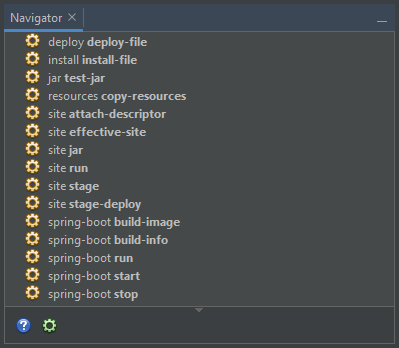
\includegraphics[scale=1]{imagens/cap10PluginsMaven}
    \\\textbf{Fonte:} Elaborada pelo autor
    \label{fig:cap10PluginsMaven}
\end{figure}
\FloatBarrier

Sendo assim, clique no nome do projeto para a aba \destaque{\textit{Navigator}} ser preenchida pelos \textit{plugins} disponíveis. De todos eles, usaremos alguns. O usado para colocar o projeto no ar, compilando-o e iniciando o servidor é o \destaque{\texttt{spring-boot run}}. Clique duas vezes nele e você verá na tela de saída o Spring Boot iniciando o processo. Se tudo der certo, você terá como última linha da saída uma mensagem informando que a inicialização foi completada. Com isso, abra seu navegador (teremos que fazer isso manualmente) e acesse o endereço \url{http://localhost:8080/}. Uma página de erro será apresentada, haja vista que ainda não temos praticamente nada dentro do nosso projeto, mas com isso já sabemos que o servidor está no ar com o projeto.

Por falar em servidor, nos Capítulos anteriores tivemos que lidar com o GlassFish lembra-se? Como estamos usando o Spring MVC como dependência, o Spring Boot usará uma versão do Tomcat, que é um container de Servlet como já aprendemos, embarcada no Spring MVC! Super legal não? Com isso não temos que nos preocupar com servidores durante o desenvolvimento da aplicação!

Vamos continuar, criando uma página index para o nosso projeto. INSTRUçÃO

\htmlCode{Arquivo \texttt{/resources/templates/index.html}}{projetos/capitulo10/venda-produtos-spring/src/main/resources/templates/index.html}

criar um index

configurar o WebConfig

\javaCode{Classe de configuração \texttt{dsoc7/vendaprodutosspring/web/WebConfig.java}}{projetos/capitulo10/venda-produtos-spring/src/main/java/dsoc7/vendaprodutosspring/web/WebConfig.java}

falar da classe VendaProdutosSpringApplication



como associar ao navegador com LiveReload

arquivo de configurações do Spring Boot

falar do POM


\section{Hibernate, JPA, Validações e Lombok}

criação das entidades
carga inicial no banco


\section{Spring MVC}

criação dos controladores e páginas com thymeleaf


\subsection{Outros \textit{Frameworks} MVC}

%Falar brevemente de: JavaServer Faces (JSF), Struts, VRaptor etc.


\section{\textit{Web Services RESTful}}

criação de controladores rest e consumir API usando Javascript.

talvez uma inserção e uma listagem?


\section{Resumo}

\section{Exercícios}

\section{Projetos}
